\section{A kétfázisú tanítási stratégia}

A modell betanítása két egymást követő fázisban zajlott. Az első fázisban (\texttt{y8x\_phase1\_960}) a YOLOv8x alap előtanított
súlyokból kiindulva, 960 képpontos bemeneti felbontáson tanítottuk be a modellt az összegyűjtött adathalmazon. A második
fázisban (\texttt{y8x\_phase2\_12803}) az első fázis legjobb súlyait (\texttt{best.pt}) töltöttük be kiindulópontként, majd
finomhangolást végeztünk 1280 képpontos felbontáson, 100 epokon keresztül. Ez a megközelítés lehetővé tette, hogy a modell
először általánosabb jellemzőket tanuljon meg alacsonyabb felbontáson, majd a magasabb felbontású finomhangolás során
részletgazdagabb mintázatokat, például finom szálhúzásokat vagy rétegcsúszásokat, is megbízhatóan felismerjen.

\section{A második tanítási fázis konfigurációja}

A második fázis főbb hiperparamétereit az alábbi táblázat foglalja össze:

\begin{table}[H]
\centering
\caption{A \texttt{y8x\_phase2\_12803} tanítási konfiguráció főbb paraméterei}
\label{tab:phase2_config}
\renewcommand{\arraystretch}{1.4}
\begin{tabular}{|l|l|}
    \hline
    \textbf{Paraméter} & \textbf{Érték} \\
    \hline
    Kiindulómodell & \texttt{y8x\_phase1\_960/weights/best.pt} \\
    \hline
    Epokszám & 100 \\
    \hline
    Bemeneti felbontás & $1280 \times 1280$ px \\
    \hline
    Batch méret & 4 \\
    \hline
    Optimalizáló & AdamW \\
    \hline
    Kezdő tanulási ráta (\texttt{lr0}) & $2 \times 10^{-4}$ \\
    \hline
    Végső tanulási ráta (\texttt{lrf}) & $0{,}01$ \\
    \hline
    Tanulási ráta ütemező & Koszinuszos csökkentés (\texttt{cos\_lr}) \\
    \hline
    Dropout & $0{,}1$ \\
    \hline
    Korai leállítás türelme & 40 epok \\
    \hline
    Adataugmentáció & Mozaik, mixup, copy-paste, RandAugment, erasing \\
    \hline
\end{tabular}
\end{table}

A tanítás során a modell automatikus adataugmentációt alkalmazott, amely magában foglalta a mozaikszerű
képösszeállítást (\textit{mosaic}), a képkeverést (\textit{mixup}, arány: $0{,}1$), a másolás-beillesztés augmentációt
(\textit{copy-paste}, arány: $0{,}2$), a RandAugment eljárást, valamint véletlenszerű törlési területeket (\textit{erasing},
$0{,}3$). A geometriai transzformációk között szerepelt $\pm10^{\circ}$-os forgatás, $0{,}7$-es skálázás, $0{,}2$-es eltolás,
valamint vízszintes és függőleges tükrözés. A magas felbontás és az erőteljes augmentációs stratégia együttesen
csökkentette a túltanulás kockázatát.

\section{Tanítási eredmények és metrikák}

\subsection{Veszteség- és metrikagörbék}

\begin{figure}[H]
    \centering
    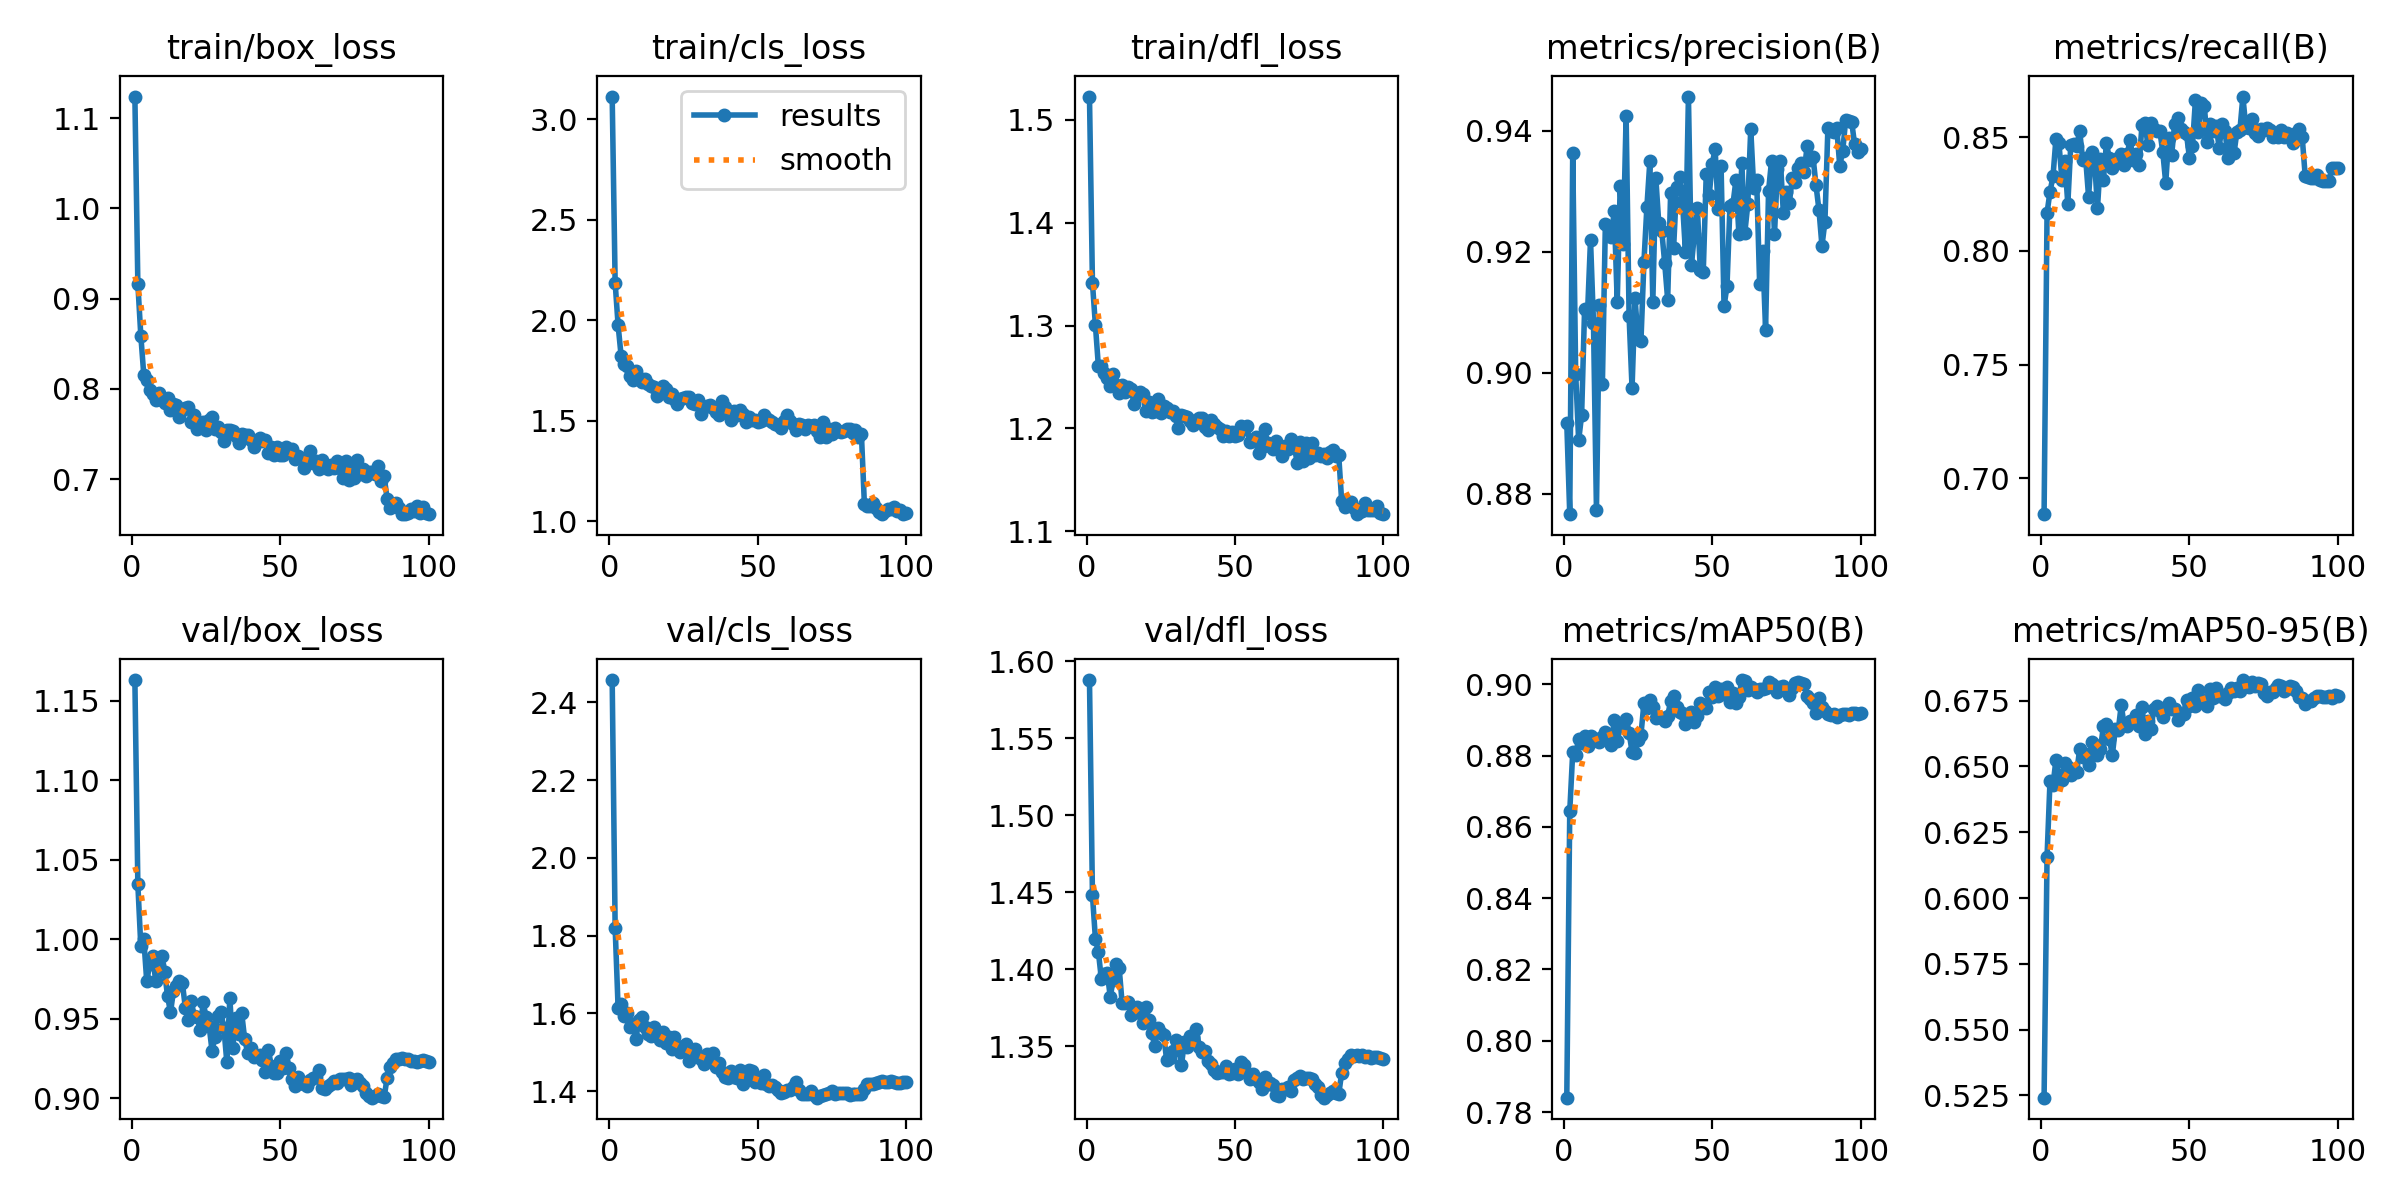
\includegraphics[width=\textwidth]{figures/images/results/y8x_phase2_12803/results.png}
    \caption{Tanítási és validációs veszteség-, valamint metrikagörbék a 100 epokon át}
    \label{fig:phase2_results}
\end{figure}

Az \ref{fig:phase2_results}. ábrán látható, hogy a tanítási és validációs veszteségek (\textit{box loss}, \textit{cls loss},
\textit{dfl loss}) mindhárom esetben folyamatosan csökkentek a tanítás során. A \textit{box loss} az első epokban $1{,}12$-ről
indult, és $0{,}66$ körüli értékre stabilizálódott, jelezve, hogy a modell egyre pontosabban jelöli ki a hibaterületeket.
A \textit{cls loss} meredekebb esést mutatott az első 10 epokban ($3{,}11 \rightarrow 1{,}71$), majd fokozatosan $1{,}04$
közelébe konvergált, ami az osztályozás gyors és megbízható javulására utal.

A validációs mAP50 metrika az 1. epokban $0{,}784$-ről indult, és a 60. epokban érte el csúcsértékét: $\mathbf{0{,}901}$.
A mAP50-95 értéke a 68. epokban tetőzött $\mathbf{0{,}683}$ értéken. A tanítás végére (100. epok) a modell
stabilan $0{,}892$ (mAP50) és $0{,}677$ (mAP50-95) körüli teljesítményt nyújtott. A koszinuszos tanulási ráta csökkentés
a 86. epokban okozott kisebb zökkenőt a veszteséggörbéken (a \textit{close mosaic} beállítás lezárása miatt), amelyet
a modell gyorsan kompenzált.

\subsection{Precision-Recall görbe}

\begin{figure}[H]
    \centering
    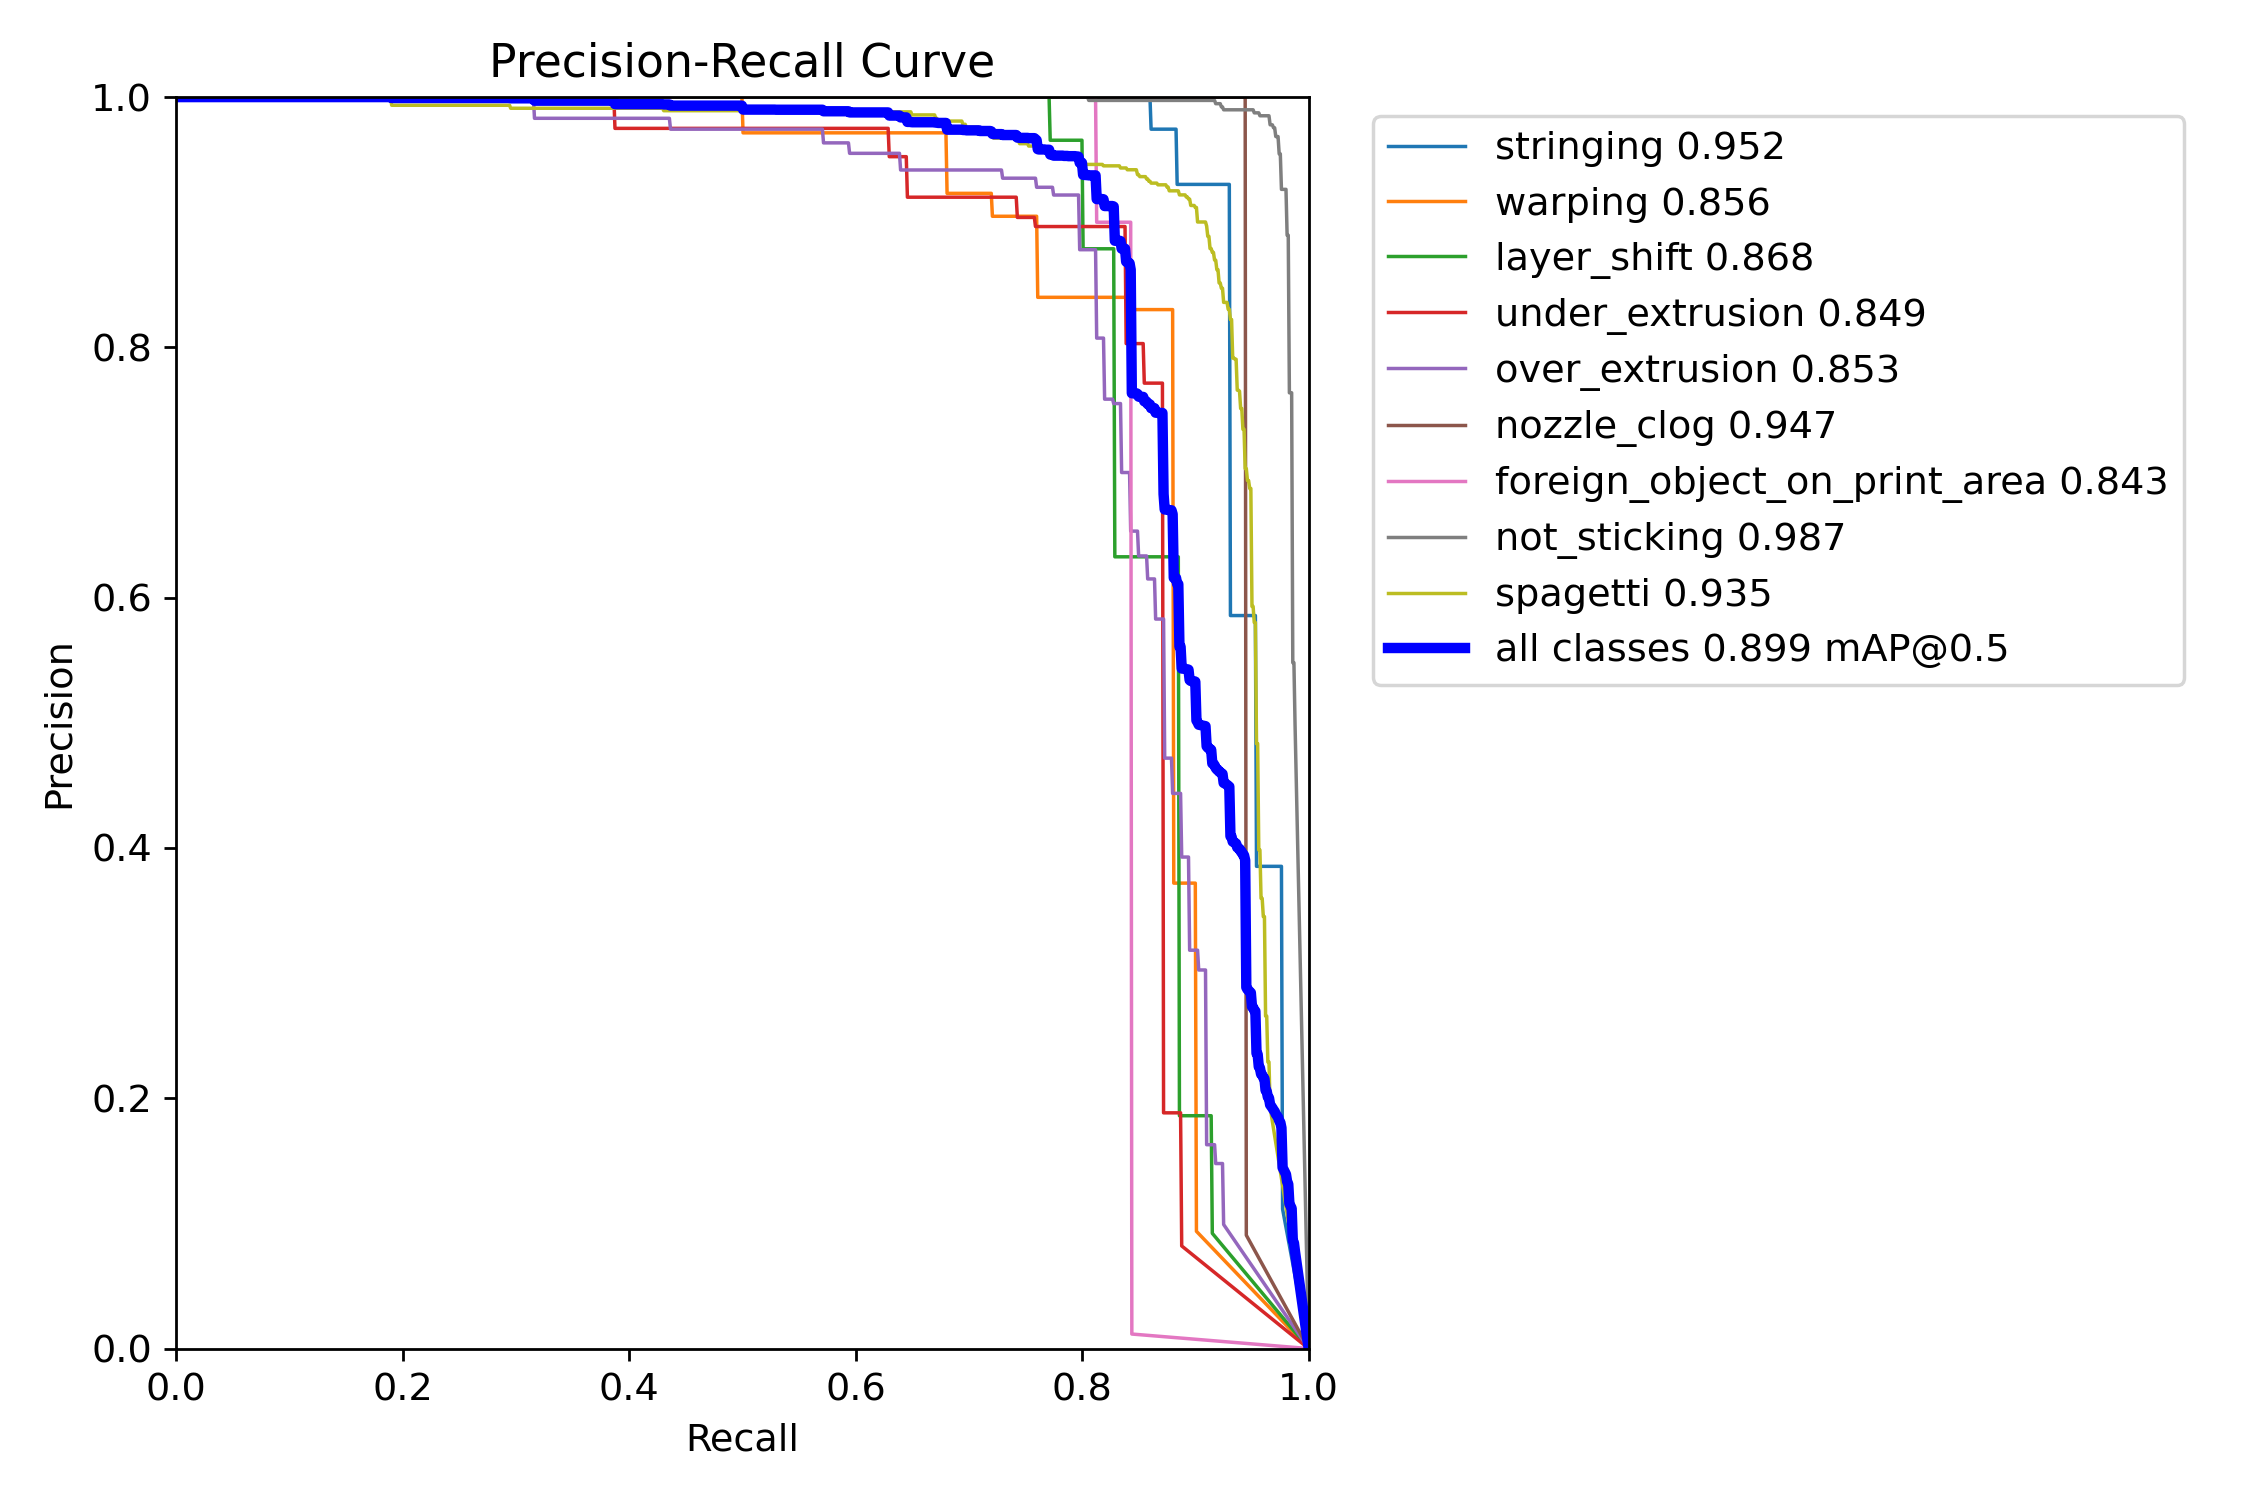
\includegraphics[width=0.8\textwidth]{figures/images/results/y8x_phase2_12803/BoxPR_curve.png}
    \caption{Precision-Recall görbe osztályonként (\texttt{y8x\_phase2\_12803})}
    \label{fig:phase2_pr}
\end{figure}

A \ref{fig:phase2_pr}. ábra az egyes hibaosztályok Precision-Recall görbéit mutatja. Az összes osztályra vonatkozó
összesített mAP@0.5 értéke $\mathbf{0{,}892}$. A görbék alapján megállapítható, hogy a modell a legtöbb hibaosztályt
magas pontossággal képes felismerni. A kisebb területű vagy vizuálisan hasonló hibatípusok, például az
\textit{under\_extrusion} és a \textit{nozzle\_clog}, esetén a görbe alatti terület alacsonyabb, ami ezeknek az
osztályoknak a nagyobb detekciós nehézségét tükrözi.

\subsection{F1-konfidencia görbe}

\begin{figure}[H]
    \centering
    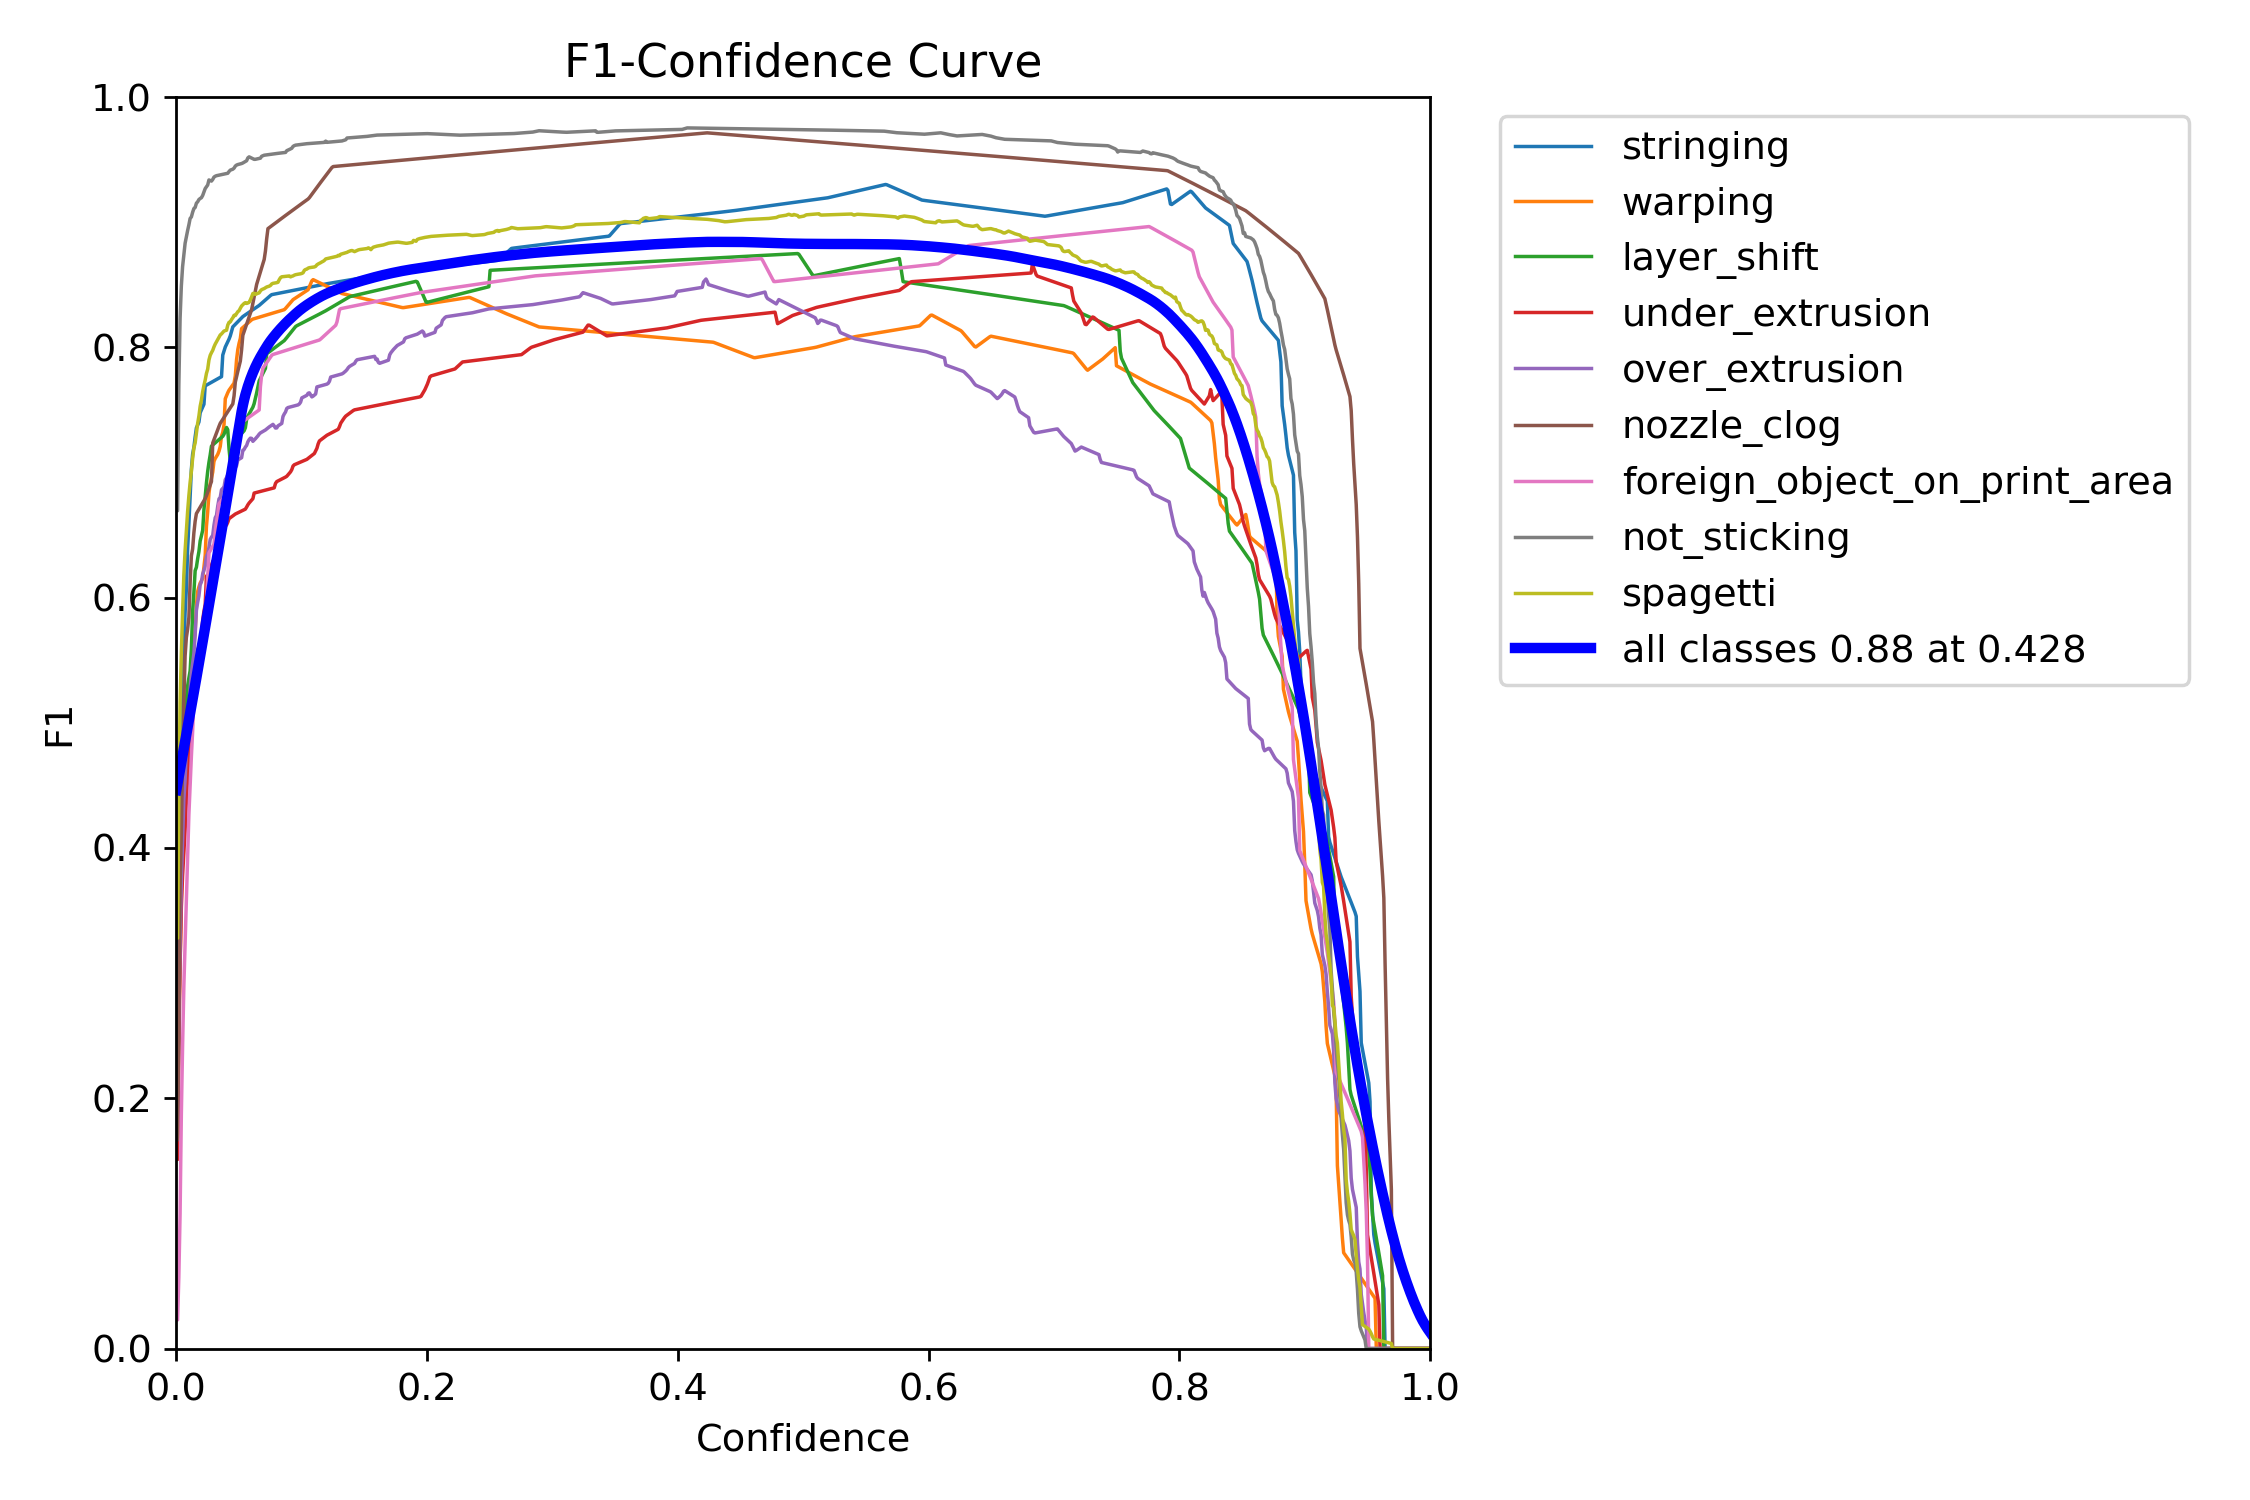
\includegraphics[width=0.8\textwidth]{figures/images/results/y8x_phase2_12803/BoxF1_curve.png}
    \caption{F1-konfidencia görbe osztályonként (\texttt{y8x\_phase2\_12803})}
    \label{fig:phase2_f1}
\end{figure}

Az \ref{fig:phase2_f1}. ábra az F1-pontszámot ábrázolja a konfidenciaküszöb függvényében. A csúcs-F1 értéke
$\mathbf{0{,}88}$, amelyet $\approx 0{,}38$ körüli konfidenciaküszöbnél ér el a modell. Ez azt jelenti, hogy a
precizitás és a visszahívási arány optimális egyensúlya ennél a küszöbértéknél érhető el az éles alkalmazásban.
A görbe viszonylag lapos a $0{,}2$-$0{,}55$ tartományban, ami robusztus viselkedésre utal a konfidenciaküszöb
finomhangolásával szemben.

\subsection{Konfúziós mátrix}

\begin{figure}[H]
    \centering
    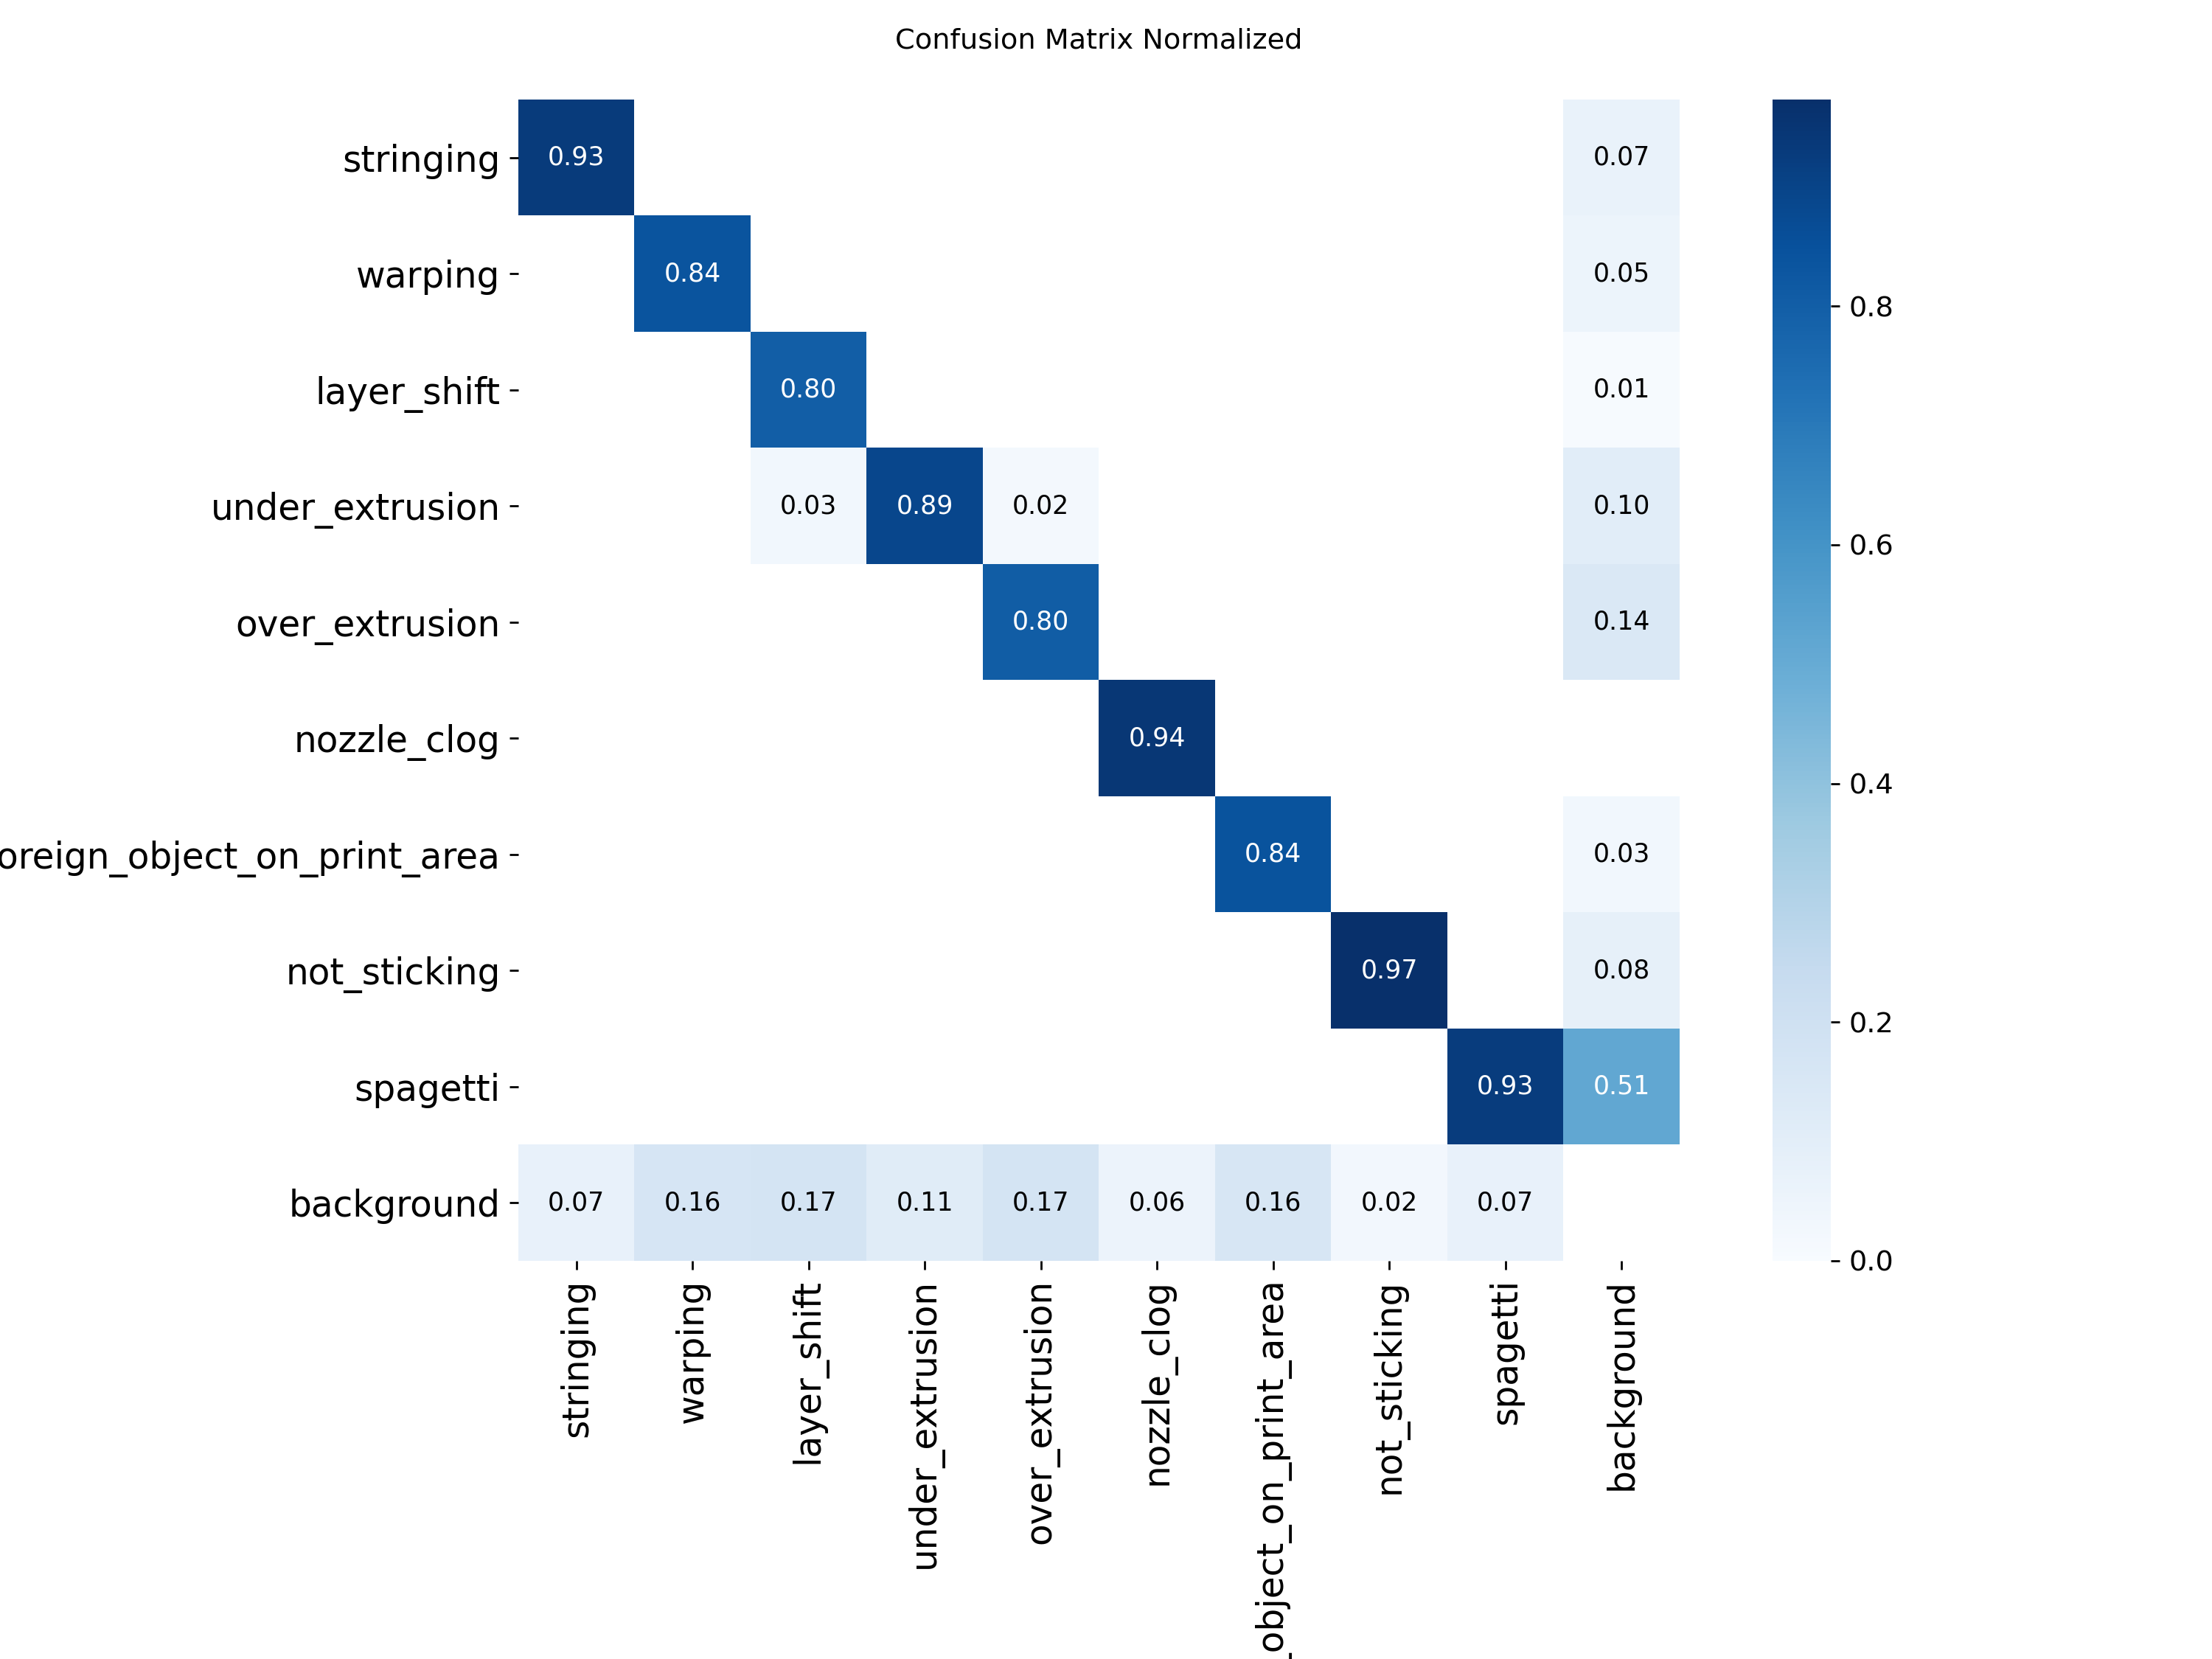
\includegraphics[width=\textwidth]{figures/images/results/y8x_phase2_12803/confusion_matrix_normalized.png}
    \caption{Normalizált konfúziós mátrix (\texttt{y8x\_phase2\_12803})}
    \label{fig:phase2_cm}
\end{figure}

A \ref{fig:phase2_cm}. ábra normalizált konfúziós mátrixa az egyes osztályok közötti tévesztések arányát mutatja.
Az átló mentén látható értékek a helyes detekciók arányát jelölik osztályonként. A mátrix alapján a modell a legtöbb
hibatípust megbízhatóan azonosítja, a \textit{background} (háttér) osztályba kerülő tévesztések főként a kisebb méretű
vagy ritkábban előforduló hibaobjektumoknál figyelhetők meg.

\subsection{Validációs predikciók}

\begin{figure}[H]
    \centering
    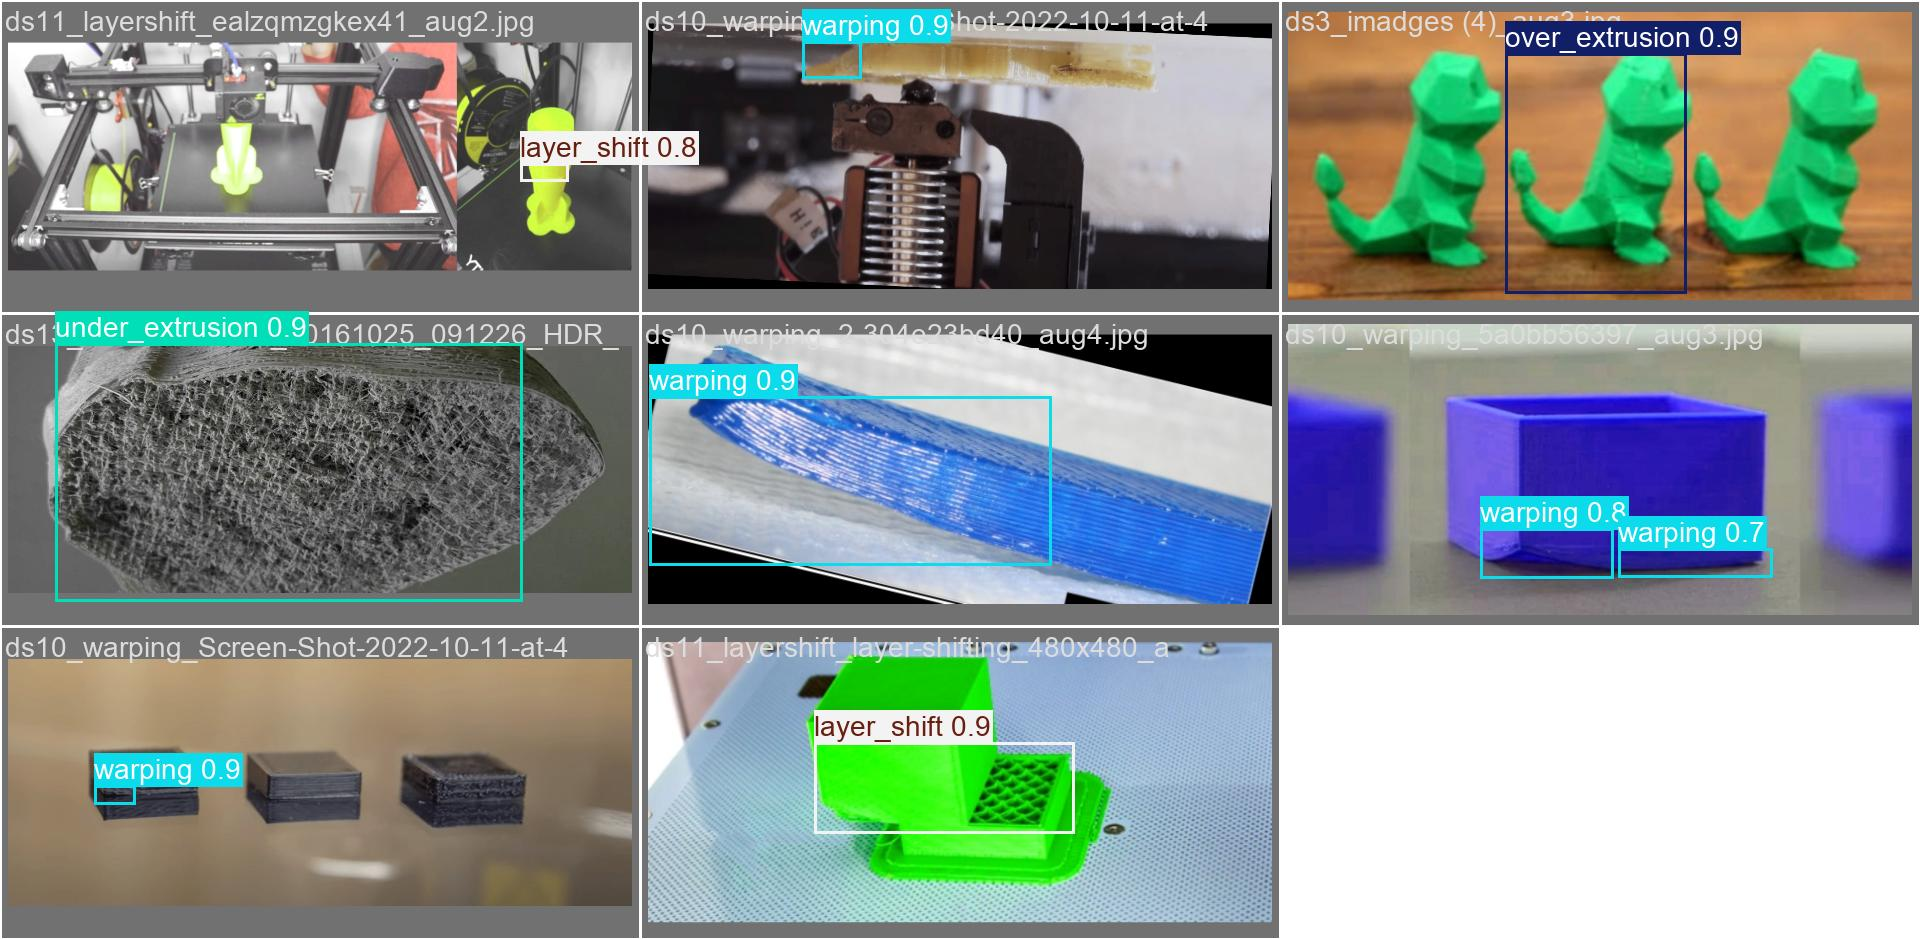
\includegraphics[width=\textwidth]{figures/images/results/y8x_phase2_12803/val_batch0_pred.jpg}
    \caption{Példa validációs batch modelljóslatok (\texttt{y8x\_phase2\_12803})}
    \label{fig:phase2_valpred}
\end{figure}

A \ref{fig:phase2_valpred}. ábra egy validációs batch modell által generált jelölődobozait mutatja. A vizuális
ellenőrzés megerősíti, hogy a modell pontosan lokalizálja és osztályozza a 3D nyomtatási hibákat, a határoló dobozok
jól illeszkednek a valós hibaterületekre.

\section{Összesített teljesítmény}

\begin{table}[H]
\centering
\caption{A \texttt{y8x\_phase2\_12803} modell végső teljesítménymutatói (100. epok)}
\label{tab:phase2_final}
\renewcommand{\arraystretch}{1.4}
\begin{tabular}{|l|c|}
    \hline
    \textbf{Metrika} & \textbf{Érték} \\
    \hline
    Pontosság (Precision) & $0{,}937$ \\
    \hline
    Visszahívás (Recall)  & $0{,}836$ \\
    \hline
    mAP@0.5               & $0{,}892$ \\
    \hline
    mAP@0.5:0.95          & $0{,}677$ \\
    \hline
    Legjobb mAP@0.5 (60. epok) & $\mathbf{0{,}901}$ \\
    \hline
    Legjobb mAP@0.5:0.95 (68. epok) & $\mathbf{0{,}683}$ \\
    \hline
\end{tabular}
\end{table}

A táblázatban összefoglalt eredmények alapján megállapítható, hogy a kétfázisú tanítási stratégia és a magas bemeneti
felbontás ($1280 \times 1280$ px) kombinációja hatékonyan javította a modell detekciós képességét. A $0{,}901$-es
csúcs-mAP@0.5 érték azt igazolja, hogy a modell megbízhatóan képes azonosítani a 3D nyomtatási hibákat valós
körülmények között is.
